\subsection{aim4.vehicle}
\label{subsec:aim4.vehicle}
\emph{aim4.vehicle} controls the different vehicles used during simulations. Vehicles are used by both \emph{Driver} and \emph{Simulator} instances. To allow them to do that the original simulator code created \emph{View} interfaces for the \emph{Driver} and \emph{Simulator} instances. Figure \ref{fig:vehicleBeforeNotA} shows how these interfaces link together. Extracting AIM behaviour was quite difficult because of how interconnected these interfaces were. The solution we came up with was to create AIM specific interfaces and link them together in a similar manner, inheriting from the generic ones if possible. Figure \ref{fig:vehicleAfterNotA} shows how the new structure links together.

\begin{figure}[htb]
\centering
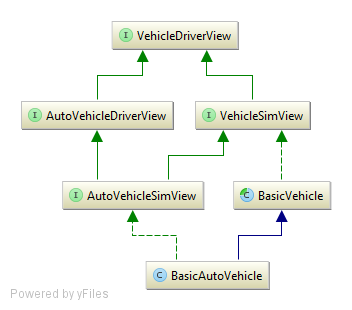
\includegraphics[width=10cm]{classDiagrams/vehicleBefore.png}
\caption{The original class structure for \emph{aim4.vehicle}.}
\label{fig:vehicleBeforeNotA}
\end{figure}

\begin{sidewaysfigure}[p]
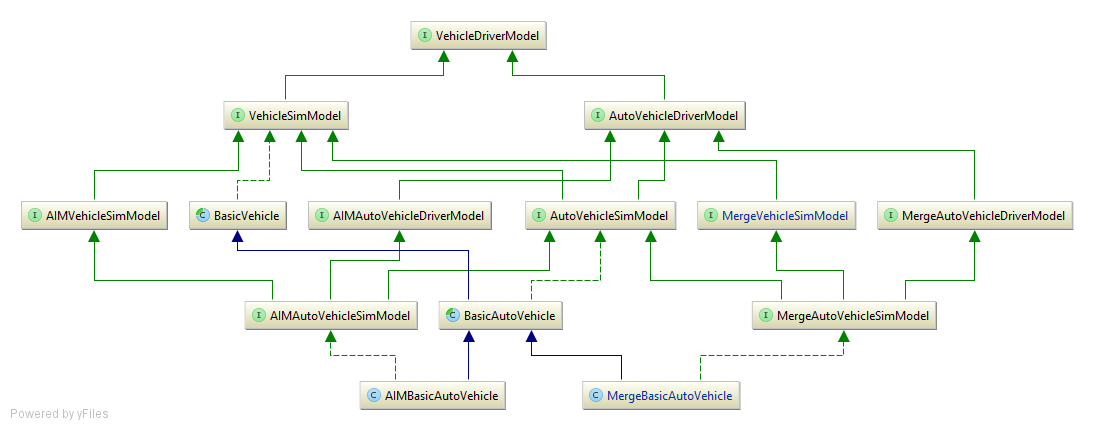
\includegraphics[width=\textwidth]{classDiagrams/vehicleAfter.png}
\caption{The new class structure for \emph{aim4.vehicle}.}
\label{fig:vehicleAfterNotA}
\end{sidewaysfigure}

The first change made to \emph{aim4.vehicle} was to rename all of the files ending in \emph{View} to end in \emph{Model} instead. We felt that \emph{View} could cause confusion with the GUI elements of the simulator; we instead chose to refer to these interfaces as \emph{Models}, because the accessors are effectively given a model of Driver and AutoDriver (beyond which they care very little) that they can use to access methods.

\emph{AIMVehicleSimModel} and \emph{AIMAutoVehicleDriverModel} are at the top of the AIM interface tree. They both extend their generic counterparts. \emph{AIMAutoVehicleSimModel} extends these two interfaces along with \emph{AutoVehicleSimModel}. This mimics the original inheritance structure. Any future vehicles will need to create their own version of these interfaces, as seen in \emph{MergeVehicleSimModel}, \emph{MergeAutoVehicleDriverModel} and \emph{MergeAutoVehicleSimModel}. 

In terms of classes we made \emph{BasicAutoVehicle} abstract and extracted out AIM specific behaviour to \emph{AIMBasicAutoVehicle}. \emph{BasicAutoVehicle} had to be abstract because we wanted to force \emph{getDriver()} to be overridden in subclasses to retrieve the simulator specific \emph{AutoDriver} for that vehicle (for example \emph{AIMAutoDriver} in AIM simulators).